\documentclass[12pt]{article}
\usepackage{graphicx}
\usepackage[margin=1in]{geometry}

\begin{document}
\title{Graph Theory \& Surface Reconstruction}
\author{Jenny Zhen}
\date{April 25, 2013}
\maketitle

\begin{abstract}The purpose of this paper is to utilize a technique for recreating models of 3-D objects. This process is referred to as surface reconstruction, which replaces a set of sample points using a faceted geometric model. Concepts of graph theory are used, specifically duals of graphs, n-regular graphs, bridgeless graphs, and matchings.
\end{abstract}

\begin{flushleft}
\section*{Introduction}
The paper will refer to the triangulation of a 3-D surface given in the figure below.

\begin{center}
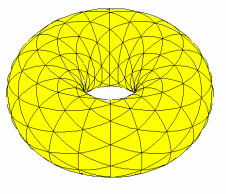
\includegraphics[scale=1]{images/torus.png}\\
Figure 1: Triangulation of a torus.
\end{center}

The figure resembles a torus, which is created by revolving a circle along a line made by another circle. Divisions of polygonal faces that form the torus produces triangular faces throughout the torus. This triangular mesh will serve as the basis for the surface reconstruction method that will be explained later in this paper.

\section*{Dual Graph}
By definition, the planar dual of any planar graph, G, can be constructed by placing a vertex in each region of G and then adding edges between regions that share a border. The planar dual is denoted as D(G).

\medskip
If a dual of the torus is to be constructed, the same procedure to create the dual of a planar graph will be used. A point will be placed in each of the triangular faces, then lines between pairs of vertices would be placed, if and only if, the corresponding faces share a common side. The dual of the torus, G, is constructed below.

\begin{center}
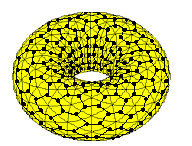
\includegraphics[scale=1.25]{images/torusdual.png}\\
Figure 2: Dual of a torus, G.
\end{center}

As shown in the figure, the triangular faces of the original torus are hexagonal faces in the dual of the torus.

\section*{n-regular Graph}
A graph is considered n-regular if every vertex in the graph is incident to exactly n edges.

\medskip
The dual of the torus is a 3-regular graph. According to the definition, that would mean that every vertex in the dual of the torus, G, is incident to exactly 3 edges. The graph of the dual is a 3-regular because each face in the original graph is a complete graph, $K_3$, in which each vertex is connected to all the other vertices. A $K_3$ graph consists of 3 vertices that all have degree 2. The dual of a $K_3$ is just one vertex inside the cycle and one vertex on the outside of the cycle, which represents the infinite region. Each edge in $K_3$ has an edge in the dual graph crossing the corresponding edge of $K_3$ to connect those two vertices, as shown below.

\begin{center}
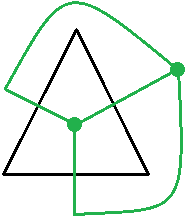
\includegraphics[scale=1]{images/k3dual.png}\\
Figure 3: Dual of a complete graph, $K_3$.
\end{center}

\medskip
By taking the dual of groups of $K_3$, a similar concept is used to connect the vertices for each region, excluding the infinite region. As a result of the three edges in each $K_3$, each vertex representing one region has three incident edges in the planar dual graph of each $K_3$. Thus, the dual of the torus is a 3-regular graph.

\section*{Bridgeless Graph}
A graph is considered bridgeless if the removal of any single edge does not disconnect the graph.

\medskip
The dual of the torus is bridgeless because the dual does not contain a cut-edge, whose removal would increase the number of components. Since the dual consists of a group of cycles, $C_6$, the edge connectivity of the dual would have to be, at minimum, the edge connectivity of $C_6$. The edge connectivity of $C_6$, $\kappa'(C_6)$, is greater than or equal to two because $C_6$ does not contain a cut-edge. As a result, the edge connectivity of the dual is at least two, as shown below.

\begin{center}
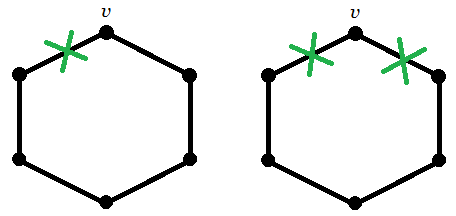
\includegraphics[scale=1]{images/c6connectivity.png}\\
Figure 4: Connectivity of $C_6$.\\
Removal of one edge in the left graph of $C_6$ does not disconnect $C_6$.\\
Removal of two edges in the right graph of $C_6$ disconnects $v$ from $C_6$.
\end{center}

\medskip
Since a grouping of $C_6$ in the dual adds one edge to each vertex, the edge connectivity of the dual is increased to three. That edge is one extra edge needed to increase the number of components. As a result, the removal of at least three edges is required to disconnect the dual of the torus. Thus, the dual of the torus is bridgeless because the removal of just a single edge does not disconnect the graph.

\section*{Perfect Matching}
A matching for a graph is a set of disjoint edges, in which no two edges share a common vertex. A perfect matching for a graph, $G$, is a set of matching edges, $M$, such that each vertex in $V(G)$ is an endpoint of some edge in $M$.

\subsection*{Petersen's Theorem}
\medskip
According to Petersen's Theorem, every 3-regular bridgeless graph has a perfect matching.

\medskip
As proven in the two sections above, the dual of the torus, G, is a 3-regular bridgeless graph. Thus, the dual of the torus must have a perfect matching.

\subsection*{Matching of a Single Face}
\medskip
Since all of the faces in the dual of the torus is a grouping of $C_6$, the matching of the dual relies on the matching of a single $C_6$. The perfect matching of a $C_6$ requires every vertex in $C_6$ to be the endpoint of an edge in the set of matching edges, $M$. This perfect matching can be created by adding every other edge in the cycle to the set of matching edges. As shown below, the set of matching edges, $M$, is $\{e_1, e_3, e_5\}$.

\begin{center}
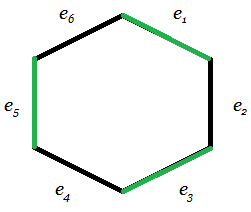
\includegraphics[scale=1]{images/c6matching.png}\\
Figure 5: Perfect matching of $C_6$.\\
Edges in the set of matching edges are colored green.
\end{center}

\subsection*{Matching of Multiple Faces}
\medskip
With a group of $C_6$, the perfect matching of the center, $center_1$, $C_6$ is the just a perfect matching of a single $C_6$ (as shown in Figure 5). The surrounding $C_6$ alternate between single $C_6$ perfect matchings and single $C_6$ with none of its edges taken as matching edges. Alternatively, it can be viewed with the center, $center_2$, being a single $C_6$ with none of its edges taken as a matching. The surrounding $C_6$ are all perfect matchings of a single $C_6$.

\newpage
\medskip
Both ways of viewing the perfect matching are below.

\begin{center}
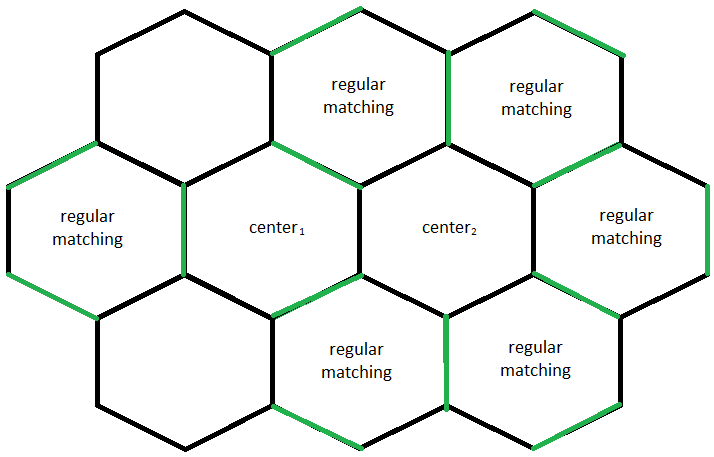
\includegraphics[scale=0.65]{images/c6groupmatching.png}\\
Figure 6: Perfect matching for a group of $C_6$.\\
Edges in the set of matching edges are colored green.
\end{center}

\subsection*{Matching of the Dual}
\medskip
Either way, the group of $C_6$ is a perfect matching because every vertex is an endpoint of an edge in the set of matching edges. Even the individual $C_6$ that do not have any edges in the matching set have every single one of its vertices as endpoints of edges in the set because its adjacent $C_6$ have already fulfilled the requirements for the vertices.

\medskip
If the groupings of $C_6$ are expanded to include all of the $C_6$ faces in the dual of the torus, there will exist a perfect matching for the dual of the torus, as shown below.

\begin{center}
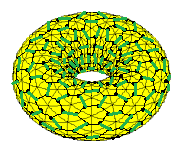
\includegraphics[scale=1.7]{images/torusmatching.png}\\
Figure 7: Perfect matching for the dual of a torus.\\
Edges in the set of matching edges are colored green.
\end{center}

\section*{B-Spline Construction}
As mentioned before, a set of sample points is collected and then fit into a triangular mesh used for the surface reconstruction.

\medskip
A method of surface reconstruction used by Matthias Eck and Hugues Hoppe is known as the B-Spline construction method. A problem with this method is that it requires quadrilateral faces instead of triangular faces. To utilize that method, the triangulation for the torus would need to be converted to contain quadrilateral faces only.

\subsection*{Face Merging}
\medskip
One method of converting triangular faces into quadrilateral faces would require the merging of faces. Pairs of faces are merged, if and only if, there is a matching edge connecting vertices in the corresponding faces. Using the perfect matching of the dual of the torus from Figure 7, the merging of the faces is drawn below.

\begin{center}
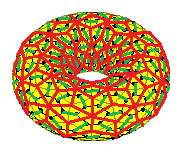
\includegraphics[scale=1.7]{images/torusmerging.png}\\
Figure 8: Face merging for the dual of a torus.\\
Edges in the set of matching edges are colored green.\\
Edges in the set of merged faces are colored red.
\end{center}

As shown above, the 3-D model of a torus is converted from a model with triangular faces to one with quadrilateral faces. The B-Spline construction method can now be used on the model of the torus.

\end{flushleft}
\end{document}